\documentclass[twocolappendix, appendixfloats, numberedappendix, twocolumn, apj]{openjournal}

\usepackage{graphicx}
\usepackage{latexsym,amssymb}
\usepackage{amsmath,morefloats}
\usepackage[backref,breaklinks,colorlinks,citecolor=blue]{hyperref}
\usepackage{natbib,graphicx,amsmath,subfigure,color,xcolor}
\usepackage{verbatim}
\usepackage{threeparttable}
\usepackage{xspace}

\newcommand{\ess}[1]{\textcolor{red}{[ESS: \bf #1]}\xspace}
\newcommand{\mrb}[1]{\textcolor{purple}{[MRB: \bf #1]}\xspace}

\newcommand{\mdet}{\textsc{metadetection}\xspace}
\newcommand{\mcal}{\textsc{metacalibration}\xspace}
\newcommand{\galsim}{\textsc{galsim}\xspace}
\newcommand{\descwl}{\textsc{WeakLensingDeblending}\xspace}
\newcommand{\ngmix}{\textsc{ngmix}\xspace}
\newcommand{\sep}{\textsc{sep}\xspace}
\newcommand{\ksigma}{\mbox{\boldmath $\mathrm{K}_{\sigma}$}\xspace}

\shorttitle{Pre-PSF Moments for Weak Lensing Shear Measurement}
\shortauthors{Becker, Sheldon, \& Rykoff}

\begin{document}
\title{Pre-PSF Moments for Weak Lensing Shear Measurement}

\author{Matthew R. Becker}
\affil{High Energy Physics Division, Argonne National Laboratory, Lemont, IL 60439, USA}
\author{Erin S. Sheldon}
\affil{Brookhaven National Laboratory, Bldg 510, Upton, New York 11973, USA}
\author{Eli Rykoff}
\affil{}

\begin{abstract}
\end{abstract}

\section{Introduction}\label{sec:intro}

\section{Pre-PSF Moment Measurement in Fourier-space}

In this section, we introduce our core methodology for computing fast, pre-PSF real-space moment
measures. It depends on the follow properties of Fourier transforms:
\begin{enumerate}
\item The Fourier transform of a quantity like $x^2W(x)$ is $\propto\frac{d^{2}W(k)}{dk^2}$.
\item The integral of the product of two functions in real-space can be computed from their Fourier
      transforms: $\int dx^2 I(x)W(x) = \int dk^2 I(k)W(k)$. This relation is called the Plancherel theorem.
\end{enumerate}
Putting the relationships together, we can compute the non-central moments of the profile of
an image via
\begin{eqnarray}
f                          & = \int dx^2 I(x)W(x) =            & \int dk^2 I(k)W(k) \\
\langle x_{i} \rangle      & = \int dx^2 x_{i} I(x)W(x) =      & \int dk^2 I(k)\frac{dW(k)}{dk_i} \\
\langle x_{i}x_{j} \rangle & = \int dx^2 x_{i}x_{j} I(x)W(x) = & \int dk^2 I(k)\frac{dW(k)}{dk_{i}dk_{j}}\,.
\end{eqnarray}
With the above we can measure pre-PSF, real-space moments as follows:

\begin{enumerate}
\item Given an image of a galaxy $I(x)$ and the PSF $P(x)$, deconvolve the PSF in Fourier-space.
\item Pick a filter function $W(x)$ that is large enough to suppress any noise from modes increased
      during the PSF deconvolution.
\item Use the relationships above to measure the moments and shape of the object through sums in Fourier-space.
\end{enumerate}

There are a fair number of technical details in the implementation that help to make it efficient and
accurate. These are discussed below.

\subsection{Weight Function Choices}

We've implemented two weight function choices. The first is a symmetric Gaussian weight
function with a given full-width-at-half-maximum. The second choice is a compact filter
in Fourier-space that we call \ksigma and was introduced by \citet{BernBFD2016}:
\begin{equation}
\label{ksigma}
W\left(|k^2|\right)  \equiv \left\{
\begin{array}{cc}
\left( 1 - \frac{k^2\sigma^2}{2N}\right)^N & k <
                                             \frac{\sqrt{2N}}{\sigma} \\
0 & k \ge
                                             \frac{\sqrt{2N}}{\sigma}
\end{array}
\right.
\end{equation}
Following \citet{BernBFD2016}, we take $N = 4$, which makes the weight a good
approximation to a gaussian.  This weight has the nice property that it goes
smoothly to zero at a chosen value of $k$. Optimizing the the measurement aperture
is non-trivial and discussed below.

\subsection{Implementation Details}

We've had to handle several technical details on the implementation in order to get
reliable and fast results. We describe and address these things one-by-one here.

\textbf{Zero-padded FFTs} The FFTs used for implementing the steps above assume that
the image is periodic. As this is never the case in real data, we zero-pad the FFTs by a
factor of four.

\textbf{Apodization} Real astronomical images can have non-zero mean background levels
due to blending of a small object on top of a larger one, errors in sky subtraction,
the bright wings of stars, etc. After zero-padding, the non-zero background level appears
as a sharp change in the image when moving over the edge of the stamp. This sharp feature
can cause artifacts in the FFTs, especially when deconvolving by the PSF. To prevent this,
we smoothly scale the image down to zero over the edge of the stamp using a cumulative triweight
apodization kernel:
\begin{equation}
T(y) = \left\{
\begin{array}{cc}
0 & y < -3 \\
(-5 * y^7 / 69984 & \\
+ 7 * y^5 / 2592 & \\
- 35 * y^3 / 864 & -3 \le y \le 3 \\
+ 35 * y / 96 & \\
+ 1 / 2) &  \\
1 & y > 3
\end{array}
\right.
\end{equation}
with $y = (x-m)/h + 3$. Here $x$ is the pixel location in the image, $m=6h$ is the maximum
apodization region, and $h$ is the kernel width parameter. This kernel is applied so that it starts
at zero at the edge of the image and goes to unity at $6h$ pixels inside the image. The exact shape
of this kernel doesn't matter as long as it is sufficiently slowly varying compared to the PSF.
We use $h=1.5$ pixels which is sufficient for a typical ground-based survey.

\textbf{PSF Deconvolution} We deconvolve the PSF in Fourier-space. In order to avoid dividing by
zero, we truncate the PSF to $10^{-5}$ of its maximum Fourier amplitude. The estimators in this work
become unstable if the moments aperture is too small in real-space and these Fourier modes are not truncated.

\textbf{WCS Handling} We require that the PSF and the image have the same WCS Jacobian
and that this Jacobian is constant across the image. We remove the WCS by mapping pixel locations
in Fourier-space to the Fourier-space WCS tangent plane before computing the moments kernels.
We correct for overall shifts in the centers of the image and the PSF though phase factors applied
in Fourier-space, but in image pixel coordinates.

\textbf{Error Propagation} We compute the errors in our measurements by directly computing the
covariance in Fourier-space. Due to the fact that all of the operations for computing the moments
above are linear, we can do this operation analytically. As shown below, our reported errors are
accurate to better than 1\% for isolated objects.

\textbf{Efficiency} Our final implementation requires two FFTs, uses \texttt{numba} to compute the
apodization masks, uses use a fast exponential implementation that is accurate to float precision,
and takes advantage of Fourier-space modes that are set to zero by the moments weight function by ignoring
them early on in the code. Overall, it runs at a speed of ${\cal O}(10s)$ of milliseconds per
object depending on the stamp size \mrb{check this again}. Our implementation is available in the
\texttt{ngmix} software package.

\section{Simulations}


\section{Results}

In this section, we focus on the results with Gaussian apertures, leaving a study of
compact Fourier-space filters to future work.

\subsection{Optimal Gaussian Aperture for an LSST-like Survey}

\begin{figure}
  \centering
  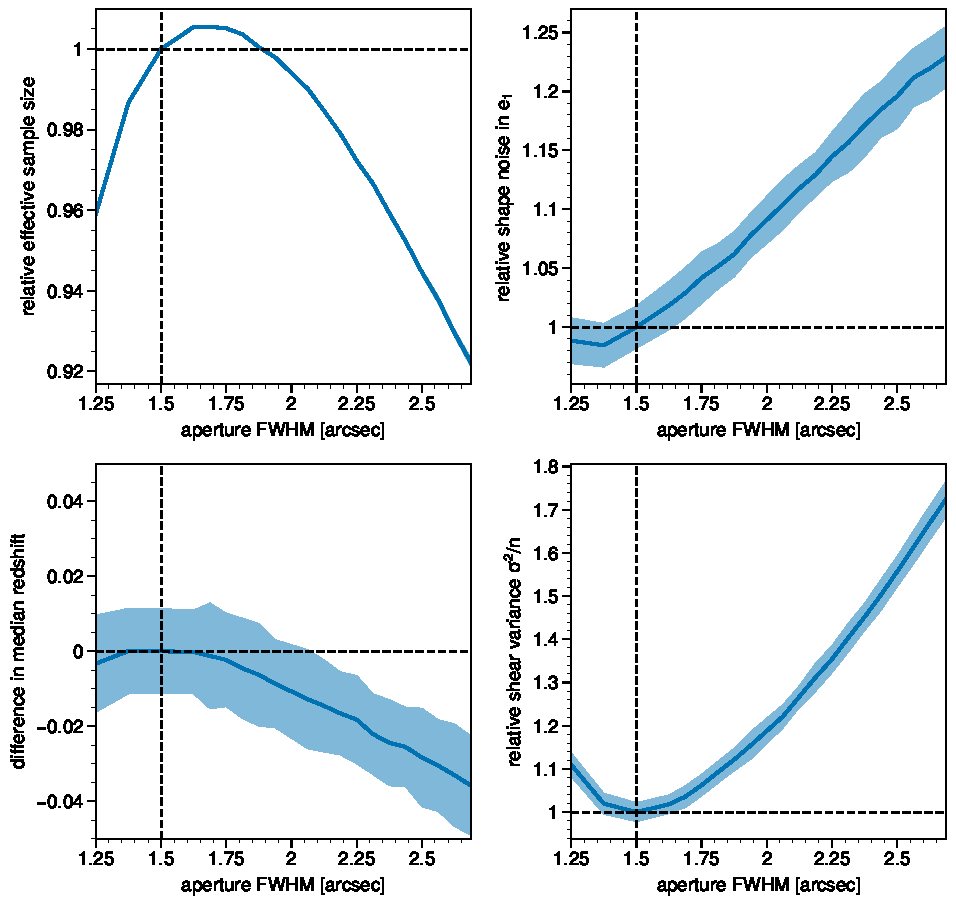
\includegraphics[width=\columnwidth]{figures/optap.pdf}

  \caption{
    Optimal Aperture for Pre-PSF Gaussian Moments. We show the relative effective sample
    size (top-left), the relative effective shape noise (top-right), the change in the median
    redshift (bottom-left), and relative total shear variance (bottom-right). All quantities are
    relative to the optimal aperture of $\approx$1.5'' FWHM. The optimum is determined by a trade-off
    between the effective shape noise and the effective number density, and it does not appear to
    result in a significant loss of redshift depth.
    \label{fig:opap}
  }

\end{figure}

We start by determining the optimal measurement aperture. For this task, we simulate
isolated objects in LSST-like $r$-band images using the \texttt{WeakLensingDeblending}
package \mrb{cite}. We then compute our moments statistics for a range of apertures between 1.25''
to 2.75''. For each aperture, we employ a set of cuts on the objects that mimics a typical weak lensing
sample selection using \mdet. These cuts are
\begin{eqnarray}
& {\rm flags} = 0 & \nonumber \\
& {\rm flux\ S/N} > 10 & \nonumber \\
& {\rm T/T_{psf}} > 0.5 & \nonumber
\end{eqnarray}
We then compute an inverse variance weight per object as
\begin{equation}
w = \frac{1}{\Delta e^2 + \sigma_e^2}
\end{equation}
where $\sigma_e$ is the raw shape noise of the sample with cuts applied and $\Delta e$ is
the pixel noise induced error on the shape measurement. Finally, we compute a set of
weak lensing sample statistics including the total sample size with cuts,
the effective number density
\begin{equation}
n_{\rm eff} = \frac{\left(\sum w\right)^2}{\sum w^2}\ ,
\end{equation}
the effective shape noise
\begin{equation}
\sigma_{e,{\rm eff}}^2 = \frac{\sum (we)^2}{\left(\sum w\right)^2}\ ,
\end{equation}
and overall total shear variance $\sigma_{e,{\rm eff}}^2/n_{\rm eff}$.

We show the results of these computations in Figure~\ref{fig:opap}. We find that the
minimal total shear variance is achieved with an aperture of $\approx$1.5'' FWHM (bottom-right panel).
In the top-left panel, we show the effective sample size scaled relative to the sample
size at the optimal aperture. We show the effective shape noise and difference in the
median redshift of the selected sample also relative to optimal aperture in the top-right and
bottom-left panels respectively. As expected, the optimal sample is a trade off between
larger apertures which increase the sample size and smaller apertures which decrease
the shape noise. We find that the median redshift of the sample has a fairly broad peak
around the optimal aperture, indicating that the optimal aperture in terms of the total
shear variance is not sacrificing redshift depth.


\subsection{Error Properties for Isolated Objects}

\begin{figure}
    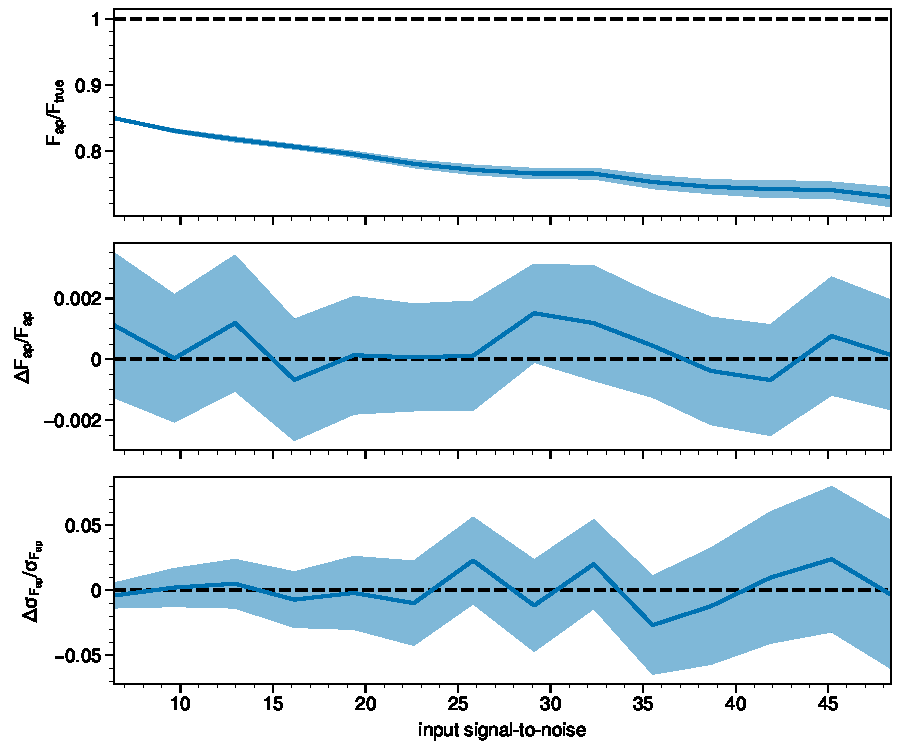
\includegraphics[width=\columnwidth]{figures/test-noround-nodetect.pdf}

    \caption{ Results of flux uncertainty measurements using \ksigma\ moments
    with perfect object detection.  In the top panel we show the fractional
    difference between the measured flux and the true flux. The flux is
    underestimated, but this is not surprising: \ksigma\ measures the flux in
    an effective aperture so the flux must be understimated. Note, however,
    that the fraction of the recovered light is independent of S/N.  In the
    middle panel we show the fractional difference between the true uncertainty
    and the predicted uncertainty.  The flux error predictions agree well with
    the true scatter in flux.  In the bottom panel we show the fraction of
    outliers identified when measuring the flux scatter.
    \label{fig:noround_nodetect}}

\end{figure}


\subsection{Shear Recovery with \mdet}

\begin{figure}
    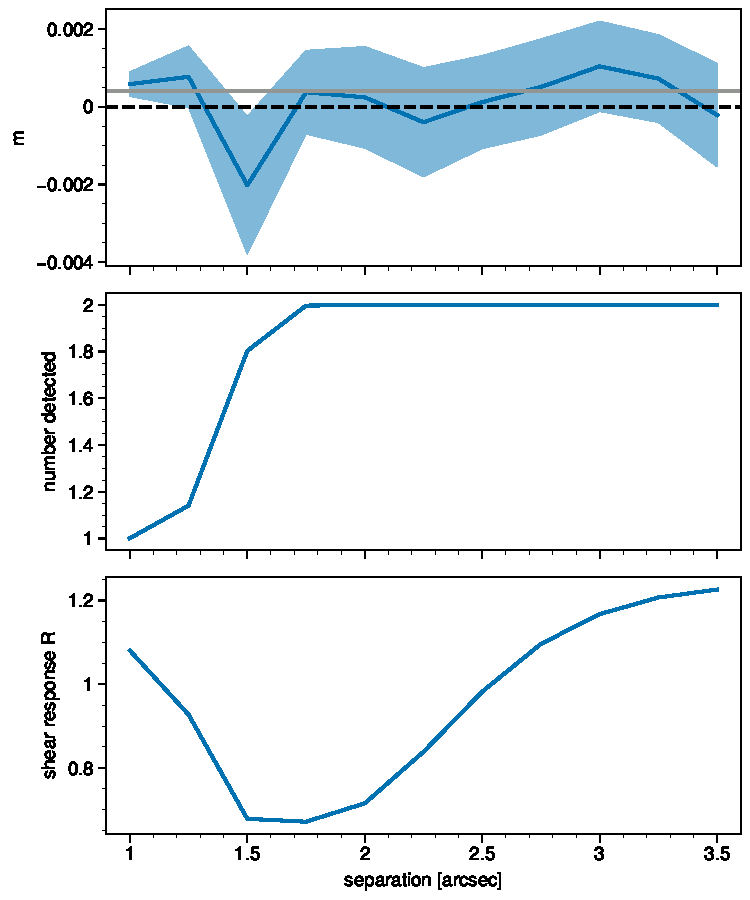
\includegraphics[width=\columnwidth]{figures/pair-plot.pdf}
    \caption{
        Tests of shear recovery for pairs of galaxies.  We compare
        \ksigma\ to a simple moment using a fixed gaussian
        weighted aperture with FWHM=1.2$''$
    }
\end{figure}

\section{Summary}\label{sec:conc}


\section*{Acknowledgments}

ESS is supported by DOE grant DE-AC02-98CH10886, and MRB is supported by DOE
grant DE-AC02-06CH11357.  We gratefully acknowledge the computing resources
provided on Bebop, a high-performance computing cluster operated by the
Laboratory Computing Resource Center at Argonne National Laboratory, and the
RHIC Atlas Computing Facility, operated by Brookhaven National Laboratory.

\bibliographystyle{aasjournal}
\bibliography{references}

% \appendix

\end{document}
